\section{检验结果\label{sec:results}}

为检验该方法的有效性，首先对介子与重子两点
关联器做了初步研究。此外，还在一个双介子系统上演示了该方法。
背景规范场由 {\em Hadron Spectrum 合作组}生成
\cite{Edwards:2008ja,Lin:2008pr}：它们是 $16^3 \times 128$
与 $20^3 \times 128$ 各向异性格点，空间与时间格距之比为 $a_s/a_t=3.5$，
含 $2+1$ 味动力学夸克。
裸轻夸克质量为 $a_t m_q=-0.0840$；当用 $\Omega$ 重子质量定标时，
对应的 $\pi$ 介子质量为 $383$ MeV。
价夸克作用量与轻动力学夸克作用量相同。

对 Sheikholeslami-Wohlert 改进离散化狄拉克方程的稀疏线性系统
进行迭代求解的数值技术在文献~\cite{Edwards:2008ja} 中描述。
特别地，这些线性系统的求解采用了 EigCG 求逆器~\cite{Stathopoulos:2007zi}。
该方法利用本征矢量降阶（deflation）来加速收敛。
最初的几次求逆调用用于构造足够好的基，
随后的求逆相比未降阶的求解器加速约三倍以上。
对于本文研究的格点，在 $N\ge 4$ 时即达到这一渐近速率。
\label{subsec:results-intro}

\subsection{蒸馏算符的轮廓分布}
    \label{subsec:results-wavefn}

蒸馏算符写成为一个向光滑场向量空间投影的低秩投影算符。
因此，几乎没有物理直觉提示它更像传统涂抹算法那样——生成大致
局域于某个束缚区域内同时保持光滑的场。
为考察该算符的性质，计算了它的空间分布。定义
\beq
   \Psi(r) = \sum_{x,t} \sqrt{\mbox{Tr } \left(\Box_{x,x+r}(t) \Box_{x+r,x}(t)
       \right)},
\eeq
则 $\Psi$ 是度量场被蒸馏算符涂抹程度的一个规范不变量。
\begin{figure}[h]
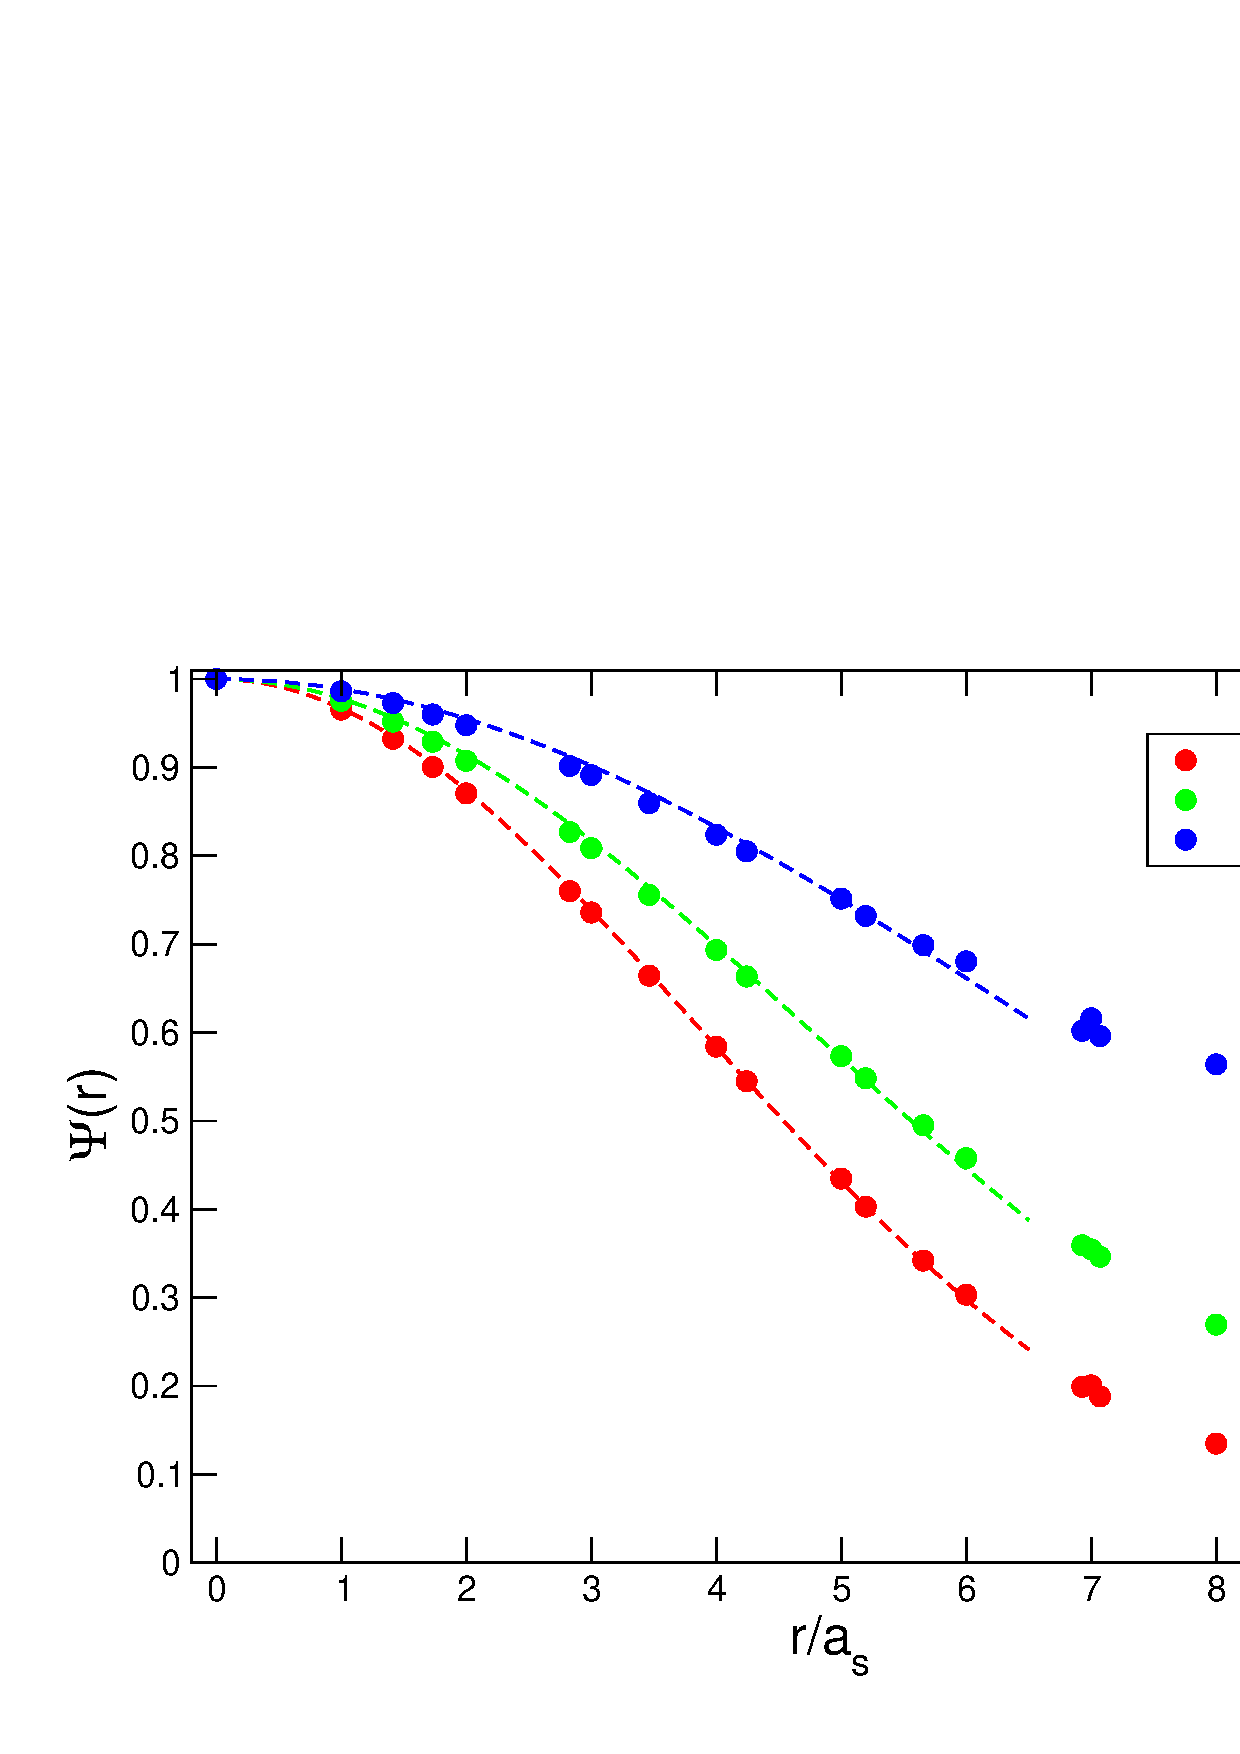
\includegraphics[width=0.6\textwidth]{images/wavefn.pdf}
\caption{\label{fig:wavefn} 由格点上拉普拉斯算符最低本征值构造的蒸馏算符的
  空间分布。数据来自 $20^3$ 空间体积，统计涨落远小于图中符号。
    虚线是对高斯分布的拟合。}
\end{figure}
该可观测量在 $20^3$ 空间格点的小系综样本上、对不同 $N$ 值及一系列
不同偏移矢量 $r$ 进行了测量，结果
示于 Figure~\ref{fig:wavefn}。数据清楚表明：
当 $N$ 在 8 到 64 之间时，蒸馏算符被高斯波函数描述得非常好。
随 $N$ 增大，该分布的半径减小。这种行为可以预料：
因为当 $N=M$ 时蒸馏算符就是恒等算符，没有任何空间延展。
Figure~\ref{fig:wavefn} 给出的测量也清楚说明
蒸馏算符具有很好的转动对称性，表明它受格点截断尺度动力学的影响极弱。
很宽的 $N=8$ 分布在较大 $r$ 处出现的伪影完全来自
这些测量所用格点的有限体积。

\subsection{介子关联函数}\label{subsec:results-mesons}

本节展示用文献~\cite{Liao:2002rj,Dudek:2007wv} 提出的基于导数的算符
构成的连通介子关联函数，重点关注 $T_1^{--}$ 道。
Fig~\ref{meff} 给出了四个对角关联器在变化蒸馏矢量数目时的有效质量图，
有效质量定义为
\begin{equation}
m_{\mathrm{eff}}(t) = - \frac{1}{\delta t} \ln \left(\frac{C(t+\delta t)}{C(t)}\right)
\end{equation}
其中 $\delta t = 5 a_t$。同时给出的还有用传统的 point-to-all 传播子构造、
分别以未涂抹源与 Jacobi 涂抹源计算的对应有效质量。
所用四个算符定义于 Table \ref{optab}。所有情形下，
算符中的规范链接均经 stout 涂抹~\cite{Morningstar:2003gk}。
此比较使用了 $16^3 \times 128$ 格点的 90 个组态。
\begin{figure*}
 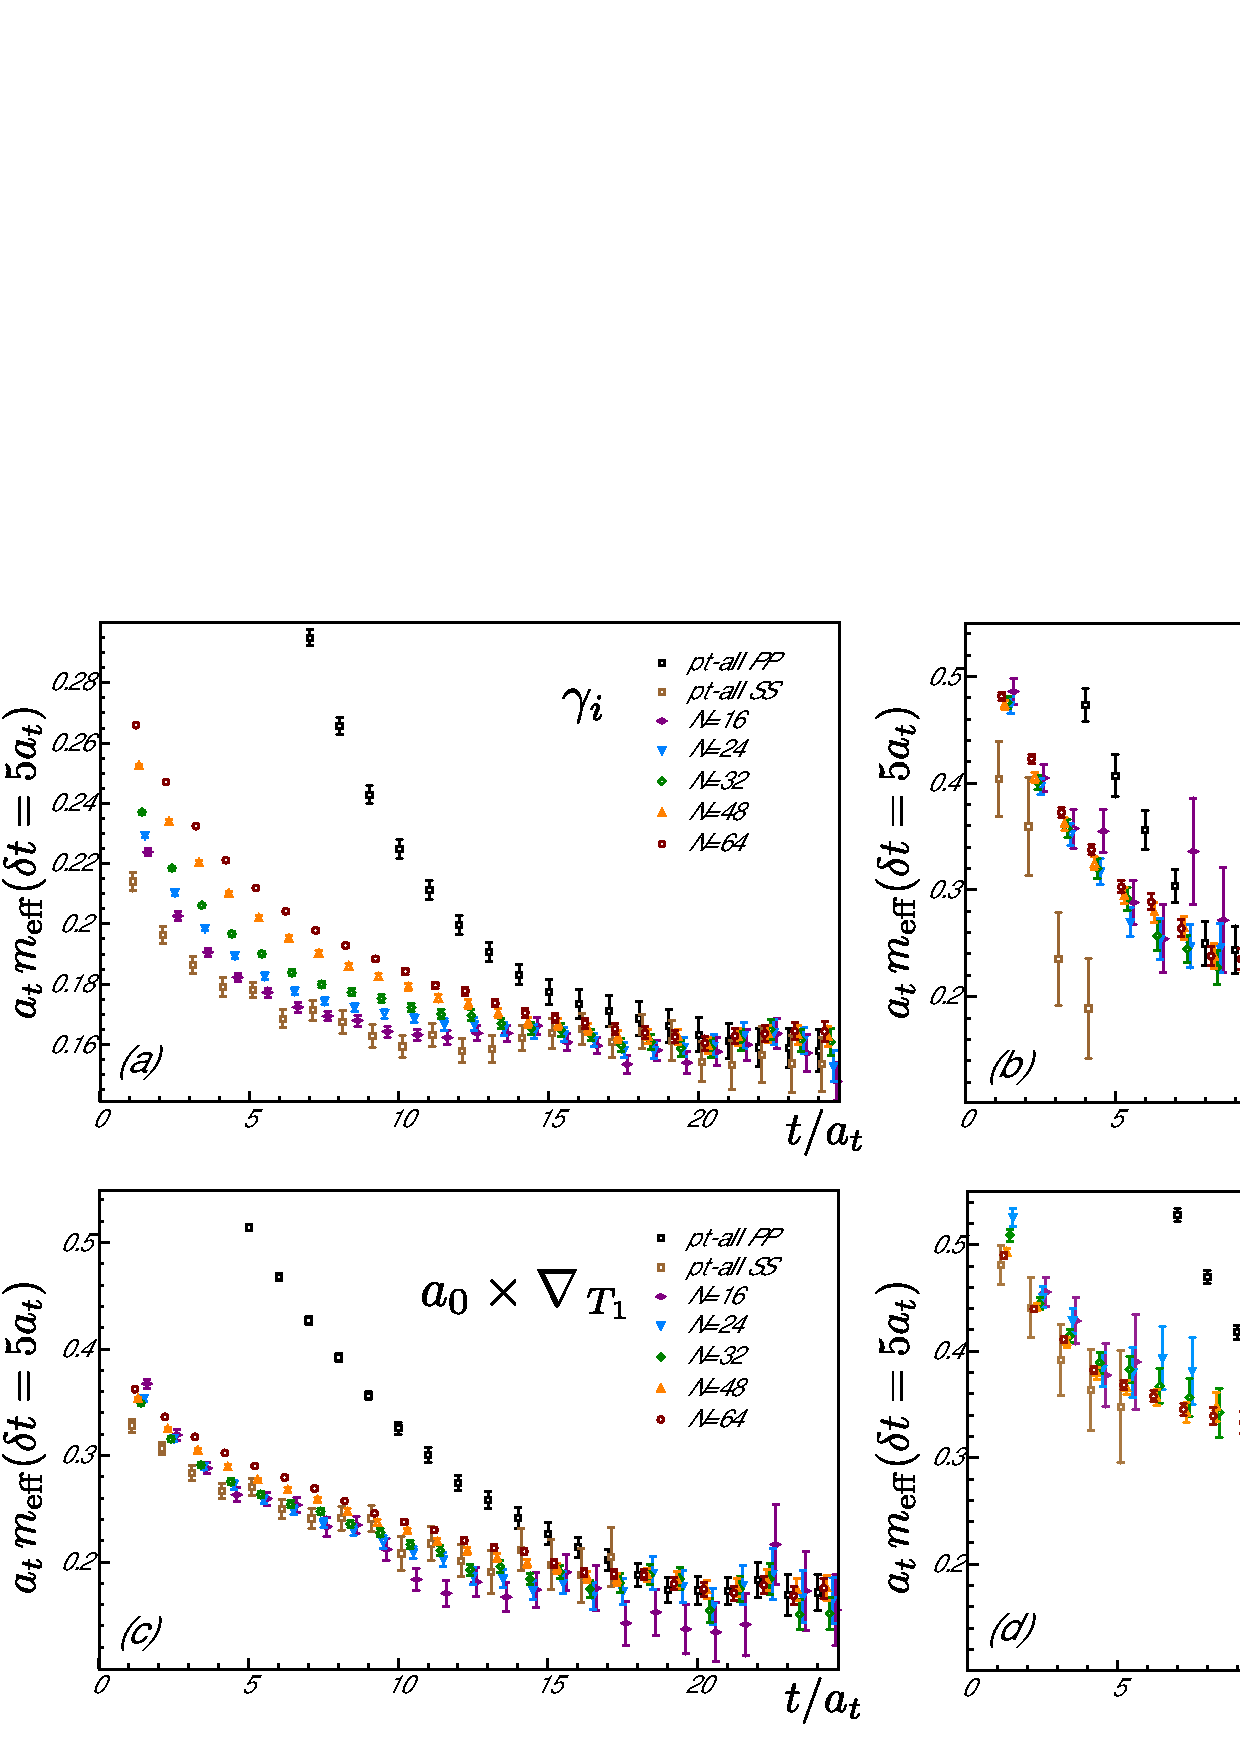
\includegraphics[width=16cm]{images/combined_notrans.pdf}
\caption{\label{meff} $16^3\times 128$ 格点上 $T_1^{--}$ 道对角关联器的
  有效质量（五时间片平移）。算符
构造见表 \protect \ref{optab}。关联器分别以 $N \in \{16,24,32,48,64\}$ 个矢量的
蒸馏夸克场构造，以及以标准规范不变夸克涂抹（SS，棕色）
与不涂抹（PP，黑色）的 point-to-all 方法构造。}
\end{figure*}
\begin{table}
 \begin{tabular}{c | c}
名称 & 构造\\
\hline
$\gamma_i$ & $\bar{\psi}\gamma_i\psi$ \\
$a_0\times \nabla_{T_1}$ & $ \bar{\psi} \nabla_i \psi$ \\
$\rho \times \mathbb{D}_{T_1}$ & $ |\epsilon_{ijk}|\, |\epsilon_{klm}|\,  \bar{\psi} \gamma_j  \nabla_l \nabla_m\psi$\\
$\pi \times \mathbb{B}_{T_1}$ & $ \epsilon_{ijk} \, \bar{\psi} \gamma_5 \nabla_j \nabla_k \psi$
\end{tabular}
\caption{\label{optab}这些检验中使用的基于导数的介子算符。
  $\vec{\nabla}$ 为单链接离散化的协变导数}
\end{table}

对两点关联函数矩阵做变分分析 \cite{Michael:1985ne,Luscher:1990ck}
已被证明是提取激发态谱与矩阵元的有力方法
\cite{Dudek:2006ej}。因此，成本估计应以构成这样一个关联器矩阵
（而非任意单个关联器）所需的计算时间为准。
作为蒸馏与传统 point-to-all 方案相对计算需求的量度，
注意在 point-to-all 方案中，
需要对原点的点源施加
    $1$、$\nabla_{i=x,y,z}$、$\nabla_i \nabla_j|_{i \neq j}$
生成的十个前向传播子，
才能产生上面定义的 $T_1^{--}$ 关联函数集。
每个这样的源需要十二次狄拉克矩阵求逆（$N_c \times N_\sigma$）。
与蒸馏方法比较时注意：大约相同的总求逆成本来自使用 32 个蒸馏矢量，因为
\begin{equation}
(N_{\mathrm{srcs}}=10) \times (N_c = 3) \times (N_\sigma = 4) = 120 \approx (N = 32) \times (N_\sigma = 4) = 128.
\end{equation}

在 $\bar\psi\gamma_i\psi$ 算符的关联函数中可以清楚地看到：
增加矢量数目使有效质量趋近未涂抹 point-to-all 关联函数的有效质量，
因为 $\sum_{k=1}^M v^{(k)} v^{(k)\dag} = 1$。
观察到统计方差随矢量数增加而迅速减小。
在该 $N$ 范围内它总是小于 point-to-all 关联器。
在 $a_0\times \nabla_{T_1}$ 道观察到类似但较慢的信号收敛。

另一方面，$\pi \times \mathbb{B}_{T_1}$ 的信号在这一矢量数目范围内
似乎基本不变，但噪声随矢量数增加而显著降低。
$\rho \times \mathbb{D}_{T_1}$ 道表现出类似行为。
注意这些算符采样了非平庸的空间依赖性，
这可能需要更大的本征矢量空间。
噪声随矢量数的快速标度可量化如下：考虑某时间片上关联器的噪信比 $r$
作为所用矢量数 $N$ 的函数，并用
\begin{equation}
r = a + \frac{b}{N^p}. \label{noise}
\end{equation}
建模。把参数拟合到最能重现来自 450 个组态的蒙特卡罗数据并在许多
时间片上平均后，得到标度指数的如下估计
\begin{eqnarray}
p(\gamma_i) = 0.8(1); \quad p(a_0\times \nabla_{T_1}) = 1.1(2); \quad
p(\pi \times \mathbb{B}_{T_1}) = 1.3(3); \quad p(\rho\times \mathbb{D}_{T_1}) = 1.8(2). \nonumber
\end{eqnarray}
所有情形中噪声降低都优于简单统计标度 $p=0.5$ 的预期。

作为对蒸馏提取激发态谱有效性的一次现实检验，
构造了一个由十二个具有 $T_1^{--}$ 量子数的算符组成的关联函数矩阵。
Figure~\ref{variational} 展示了提取的低躺谱随所用矢量数的变化。
\begin{figure}[h]
 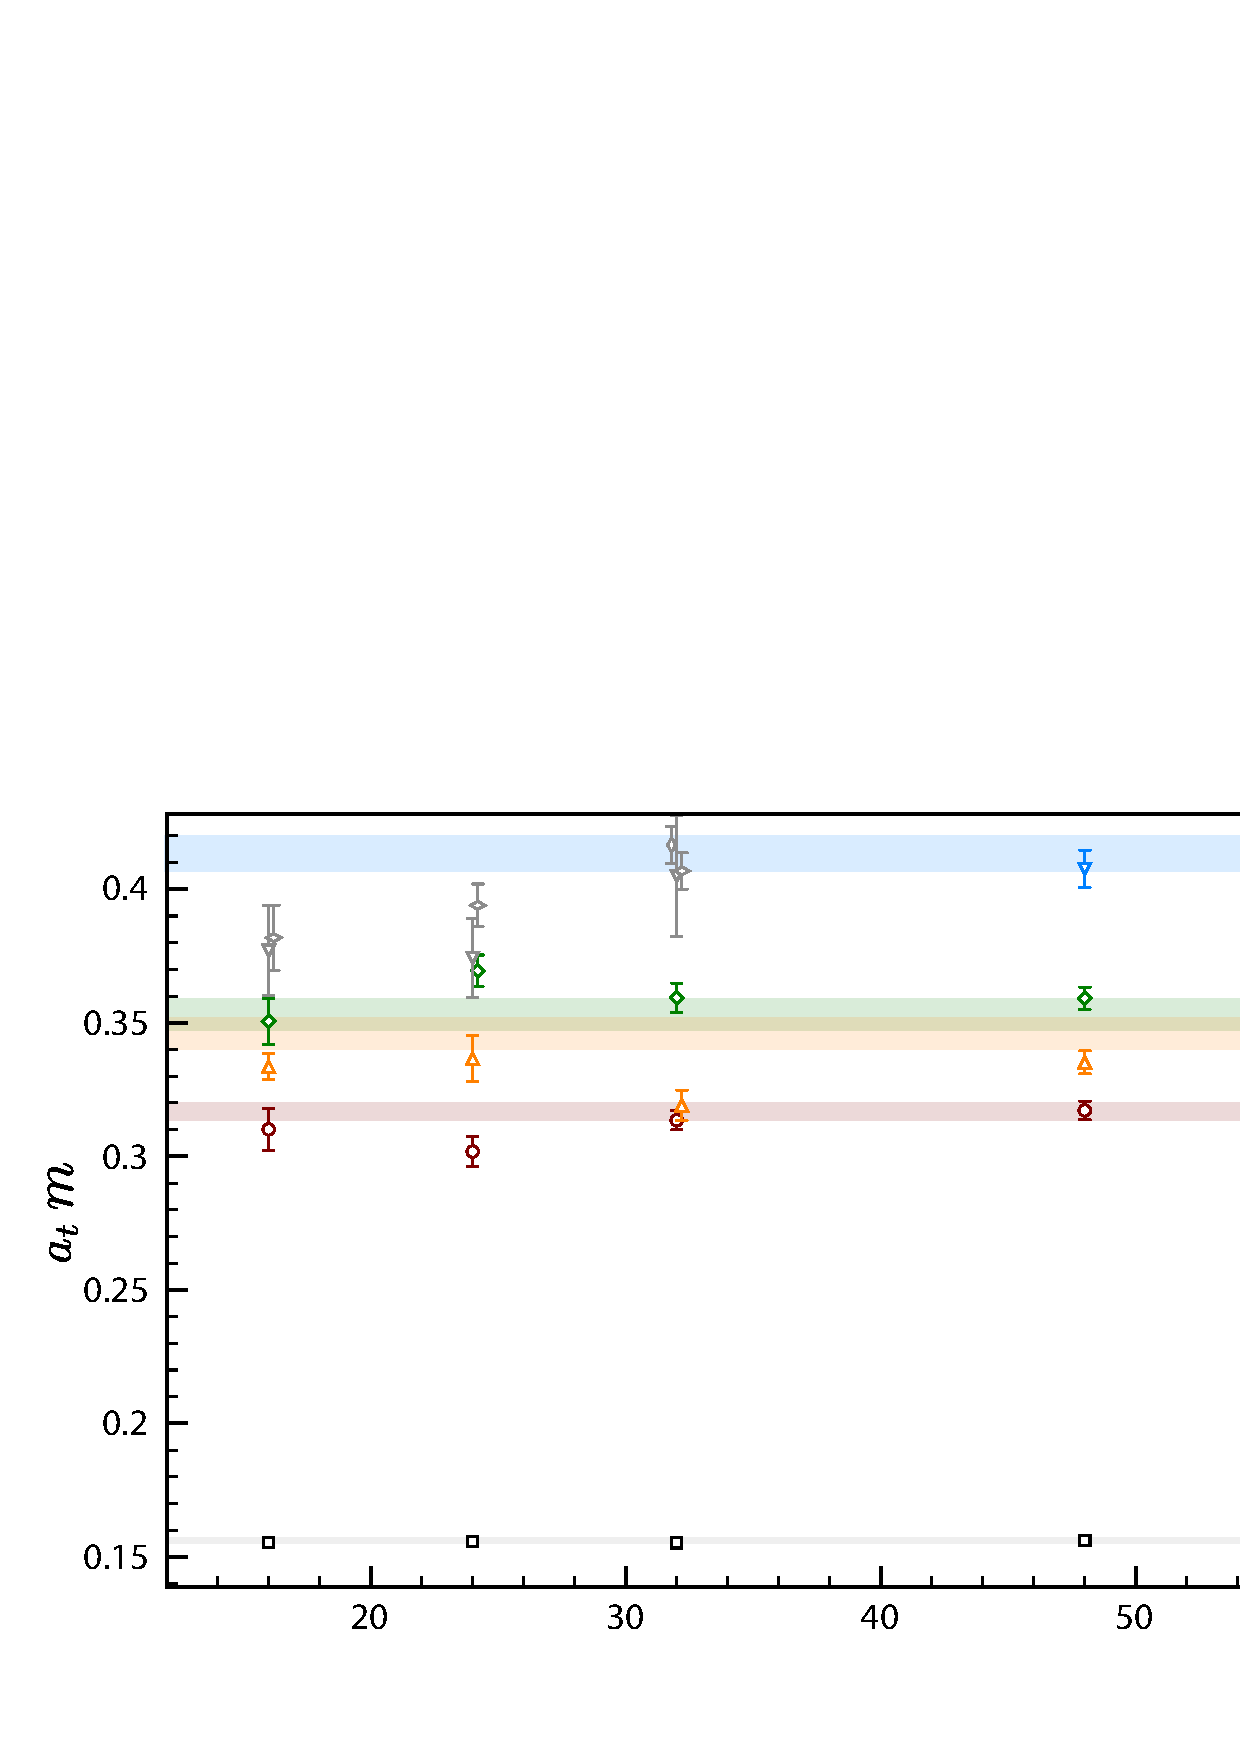
\includegraphics[width=12cm]{images/variational_16.pdf}
\caption{\label{variational} $T_1^{--}$ 变分质量谱随所用本征矢量数目的变化。
误差棒纯属统计误差，未计入拟合可能带来的系统误差。   }
\end{figure}
显然，
即便用相对较少的矢量，该方法也能用于构造两点关联矩阵，
并从中以一定精度提取低能态谱。
直到第四激发态的质量都随矢量数增加而变得更加一致。

现在考虑该方法随格点体积增大的标度问题。
Figure~\ref{voltest} 展示了分别在 $16^3$ 与 $20^3$ 格点上计算的
关联器有效质量，此处空间体积比非常接近 2（$\tfrac{20^3}{16^3} = 1.95$）。
显然，$16^3$ 体积上用 $N$ 个矢量的关联函数与 $20^3$ 格点上
用 $2N$ 个矢量的情形基本相同。注意：虽然格点体积从 $16^3$
增至 $20^3$ 时同一信号的求逆次数翻倍，
但噪声降低了约两倍。

对这一效应一个非常简洁的解释来自考察拉普拉斯算符的这些本征矢量
所属的本征值，
$\nabla^2 v^{(k)} = - \lambda_k v^{(k)}$。Figure~\ref{evals}(a) 展示了
在 $16^3$ 与 $20^3$ 格点上测得的本征值。可以考虑这样选取蒸馏算符的秩：
使用本征值低于某个截断的所有本征矢量。
从图中清楚可见，在更大体积上这将需要更多本征矢量。
Figure~\ref{evals}(b) 更直接地显示了本征值小于截断的本征矢量数。
$20^3$ 情形所需的本征矢量数约为 $16^3$ 情形的两倍才能达到同样的截断。
从这一分析看来，介子关联器信号实际上由构造蒸馏空间所用
本征值的截断决定。
这等价于用 Heaviside 近似来做涂抹：
$J_{\lambda}(t) = \Theta( \lambda + \nabla^2(t)  ) = \sum_{k=1}^M \Theta(\lambda -  \lambda_k )  v^{(k)}(t) v^{(k)\dag}(t) = \sum_{k=1}^{N(\lambda)} v^{(k)}(t) v^{(k)\dag}(t).$



\begin{figure*}
 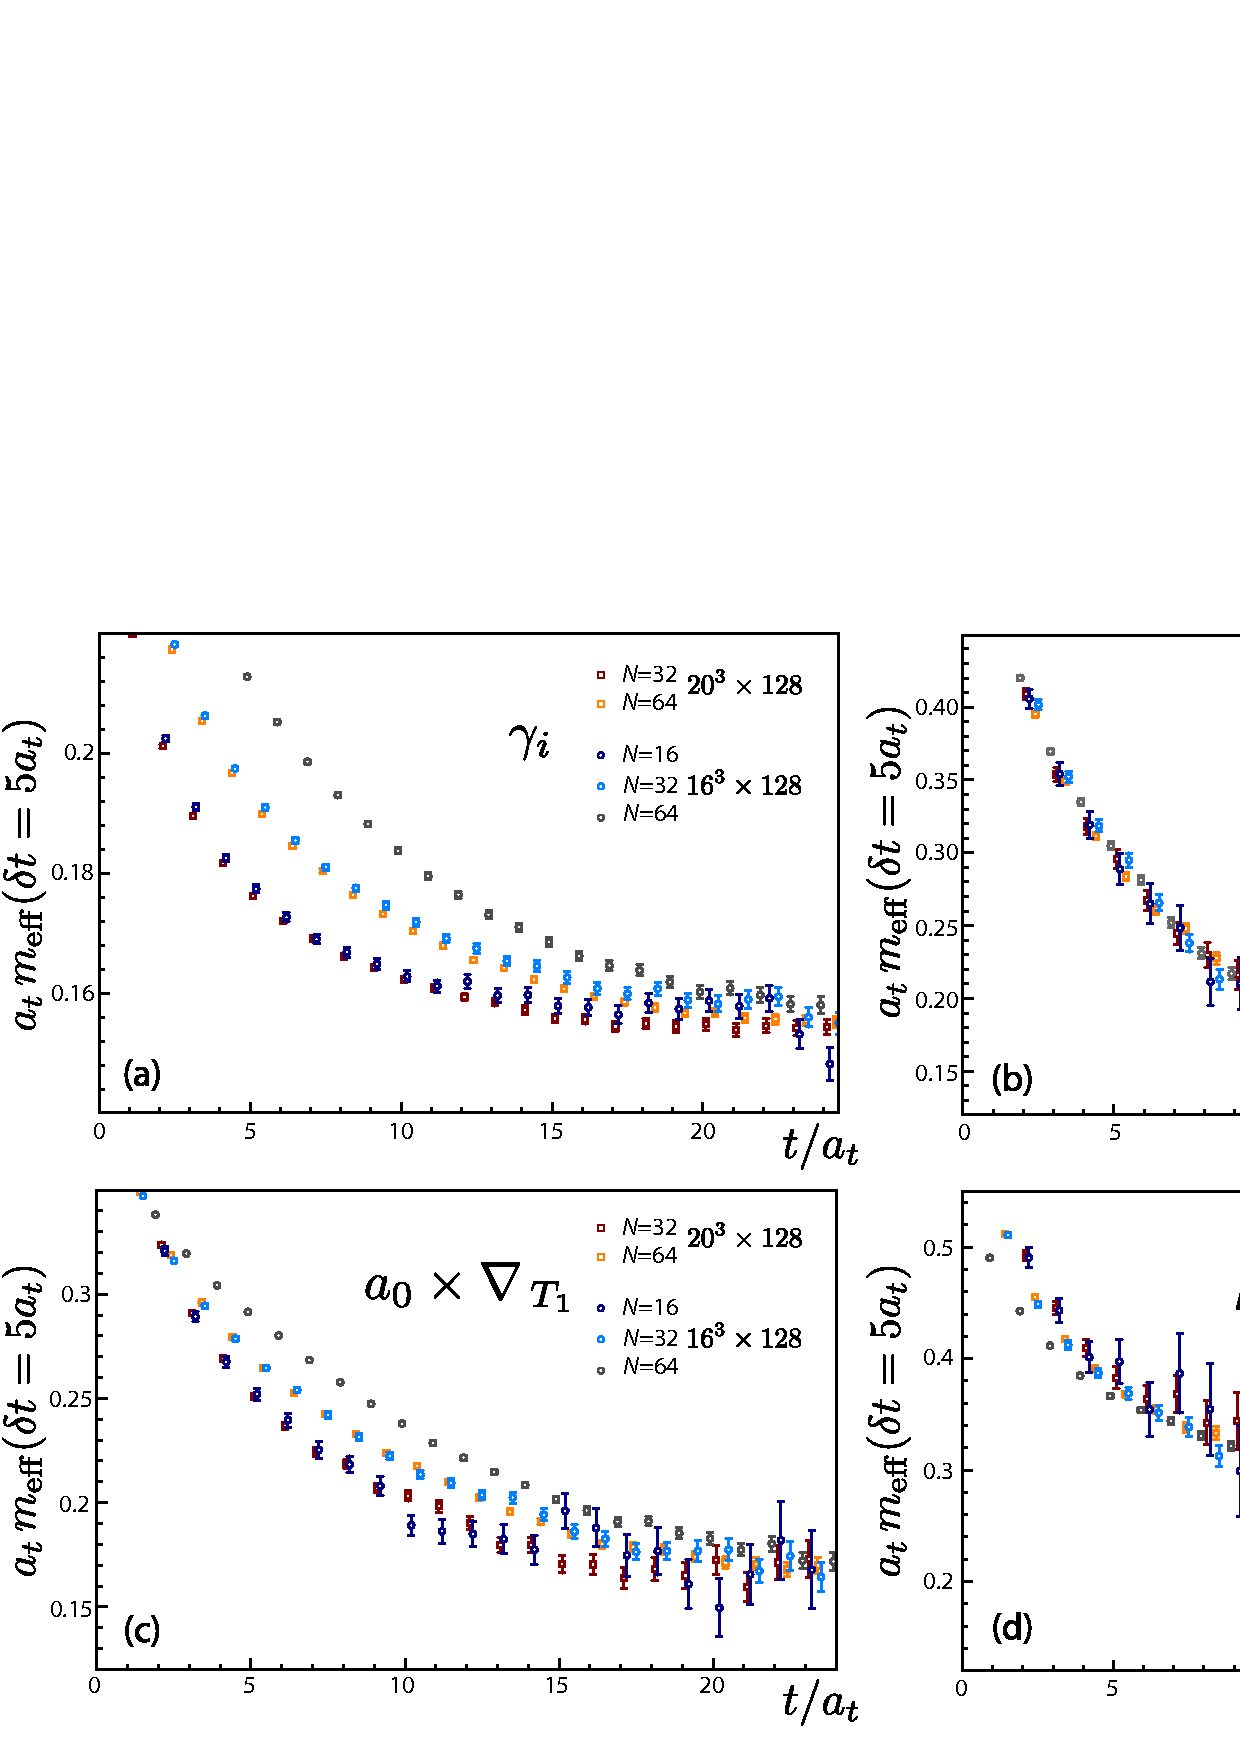
\includegraphics[width=16cm]{images/combined_16vs20.pdf}
\caption{\label{voltest} $16^3$ 与 $20^3$ 空间体积上 $T_1^{--}$ 道对角关联器的
有效质量（五时间片平移）。算符构造见表
\protect \ref{optab}。}
\end{figure*}

\begin{figure*}
 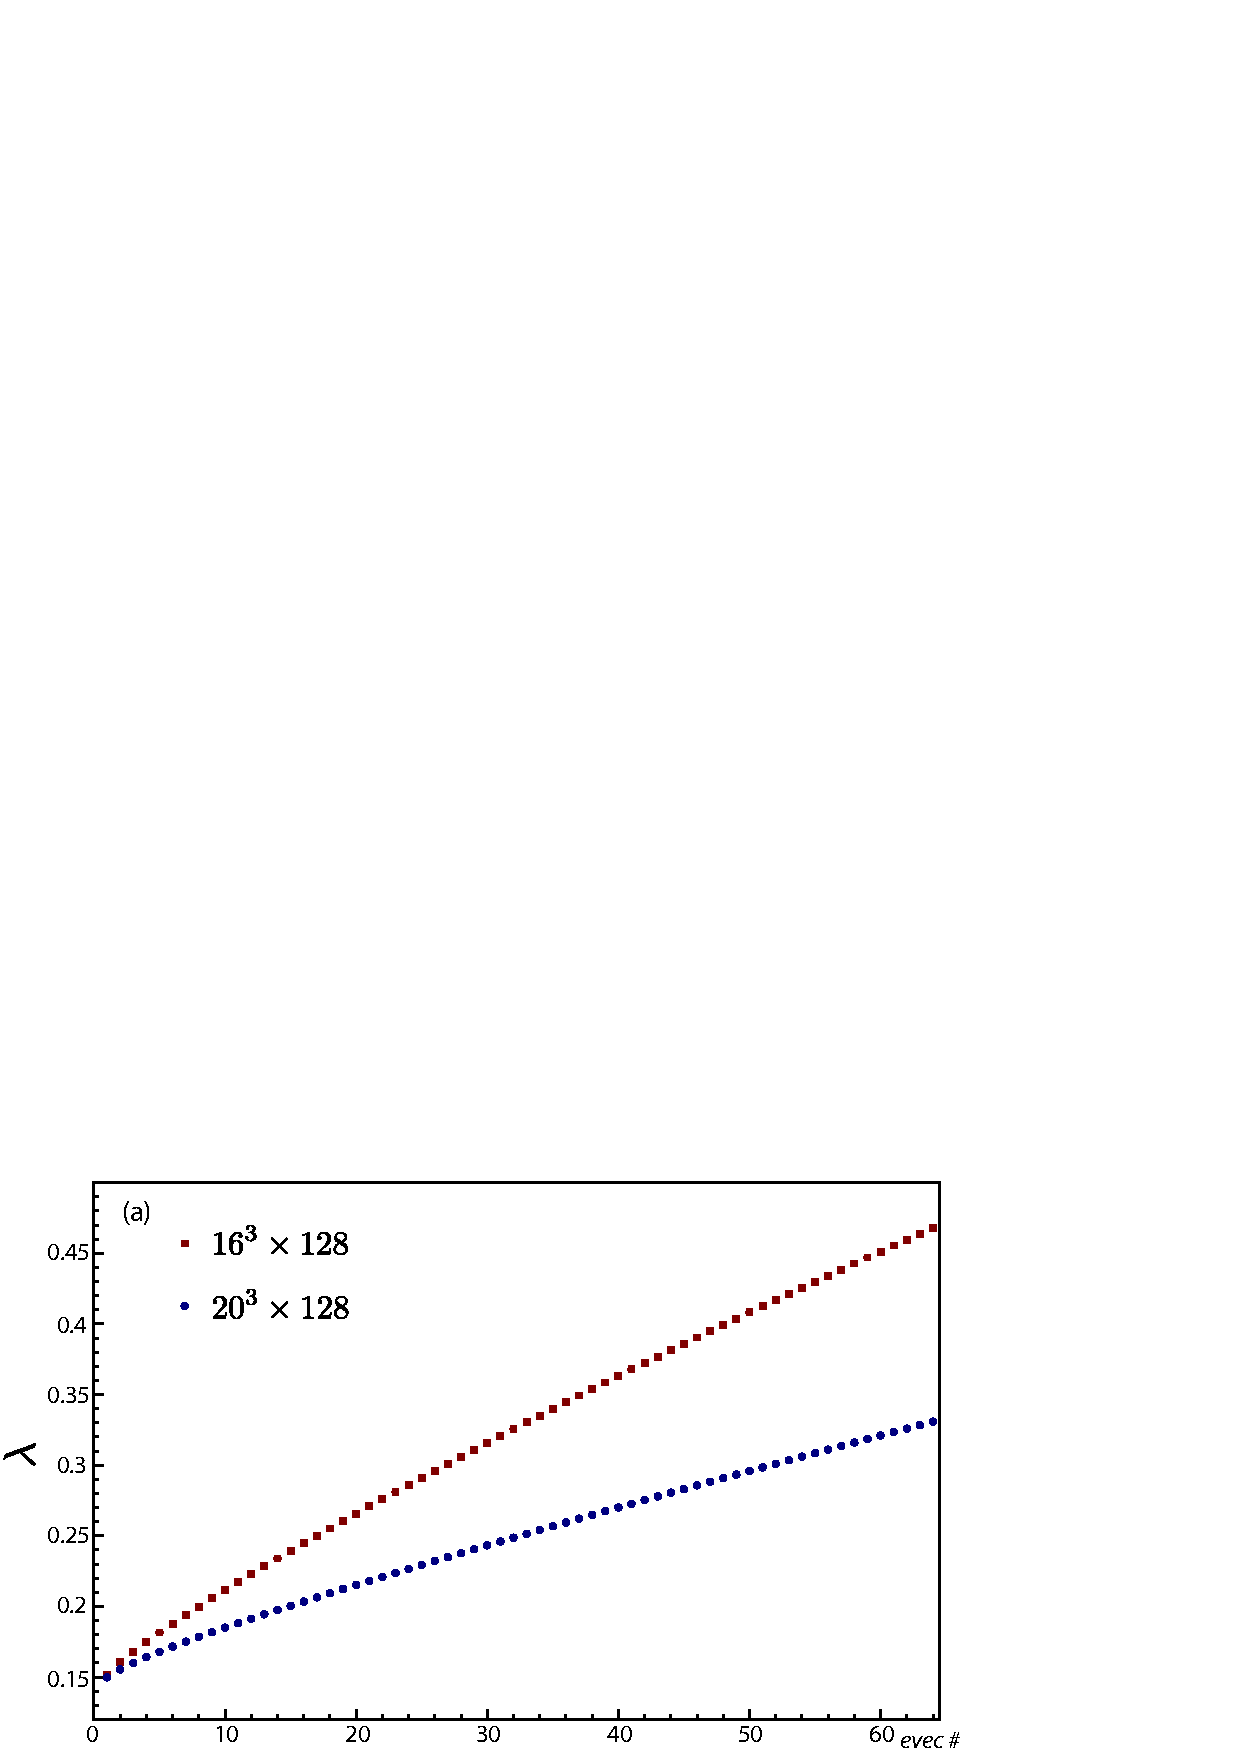
\includegraphics[height=5cm]{images/evals_edited.pdf}
\hspace{5mm}
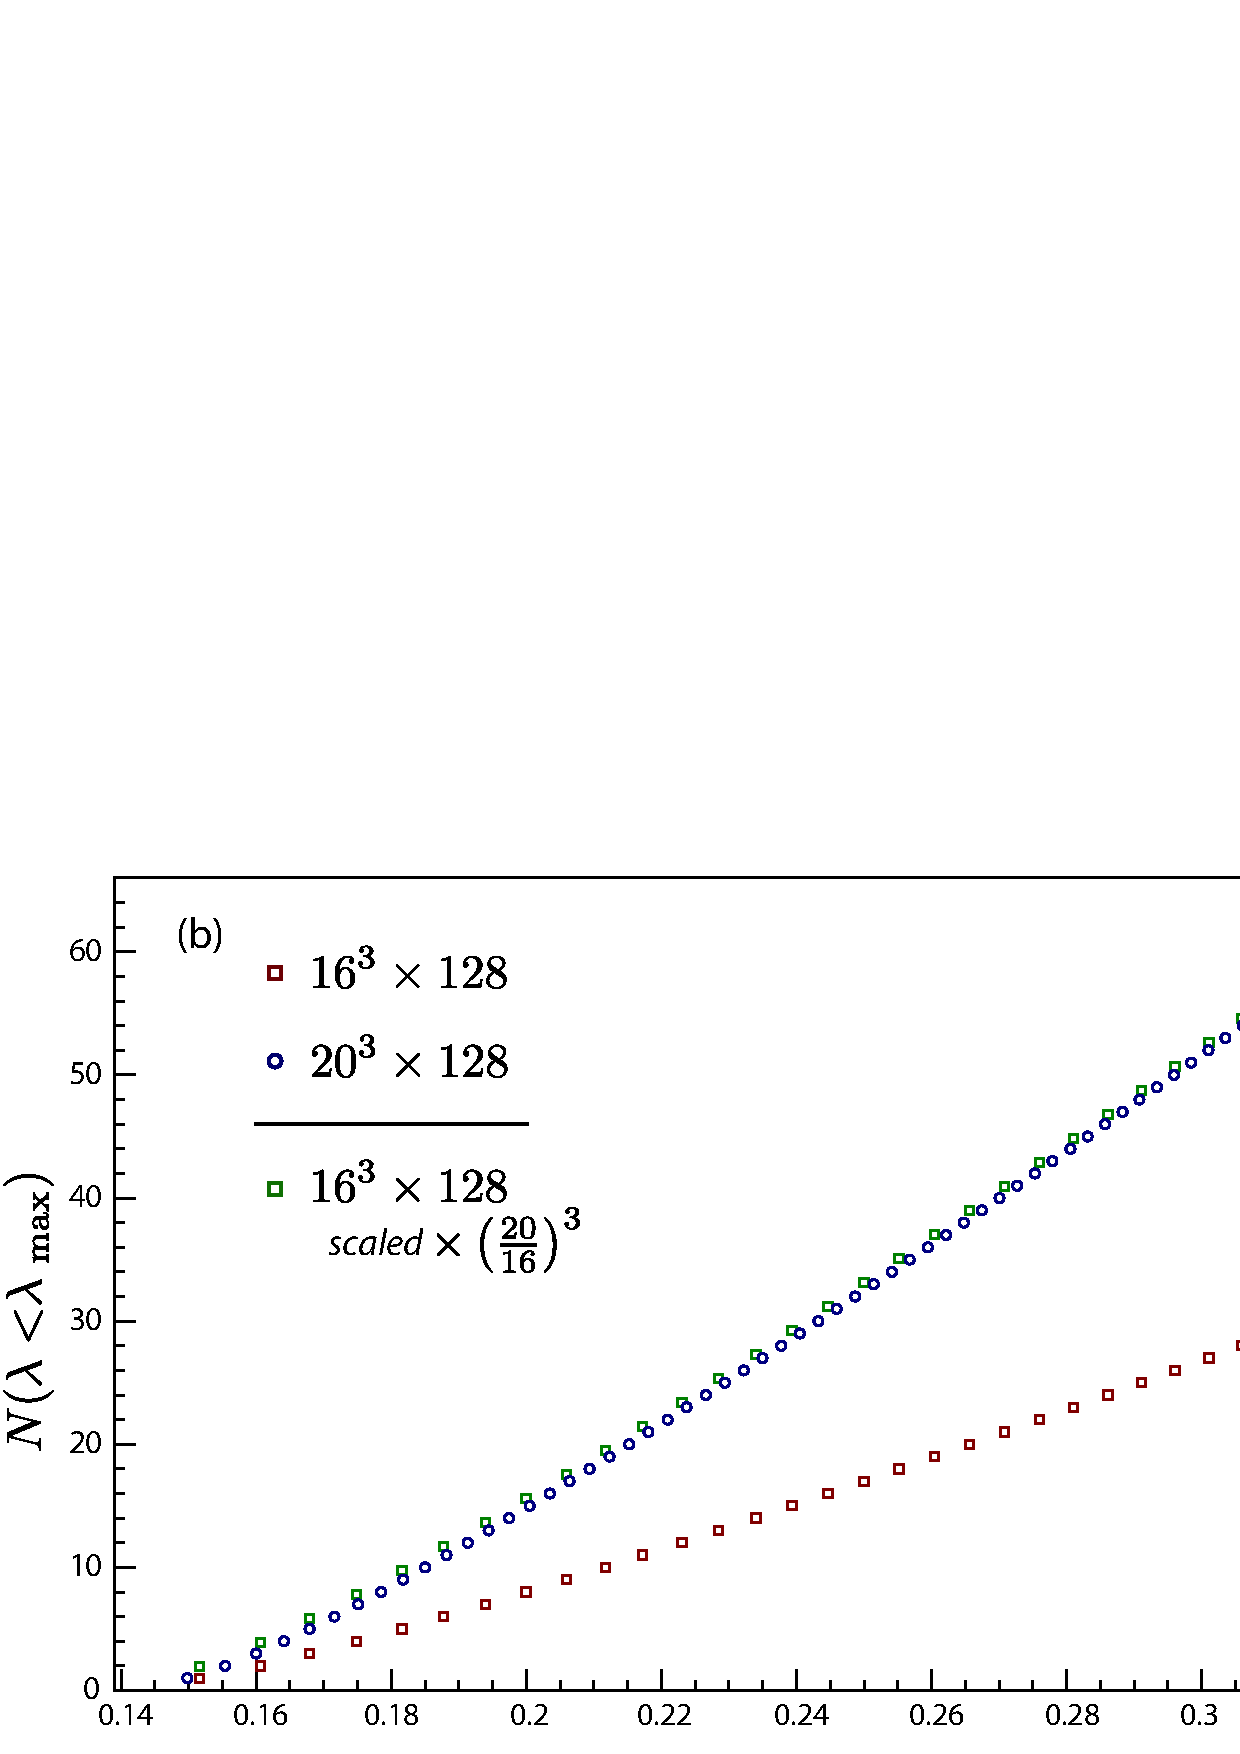
\includegraphics[height=5cm]{images/cutoff_new_edited1p95.pdf}
\caption{\label{evals} (a) $16^3$ 与 $20^3$ 格点上拉普拉斯算符的本征值。(b) $16^3$ 与 $20^3$ 上本征值低于 $\lambda_{\mathrm{max}}$ 的本征矢量数。同时给出按因子 $\left(\frac{20}{16}\right)^3$ 缩放的 $16^3$ 数据。  }
\end{figure*}

\subsection{重子关联函数}\label{subsec:results-baryons}

重子关联函数采用文献~\cite{Basak:2005aq,Basak:2005ir} 描述、
并在谱研究~\cite{Basak:2007kj, Bulava:2009jb} 中使用的位移夸克算符计算。
在四个核子 $G_{1g}$ 算符上演示了蒸馏方法：
其中两个局域在单个格点，其余两个带单位移夸克场。
相应的 $4 \times 4$ 关联器矩阵在 $16^3 \times 128$ 格点的 316 个组态上计算。
Figure~\ref{fig:baryon_meff_Nev} 给出对角关联器的有效质量图。
观察到清晰的趋势，与介子情形类似：
随本征矢量数增加，关联器的激发态贡献增大而统计涨落减小。
\begin{figure}
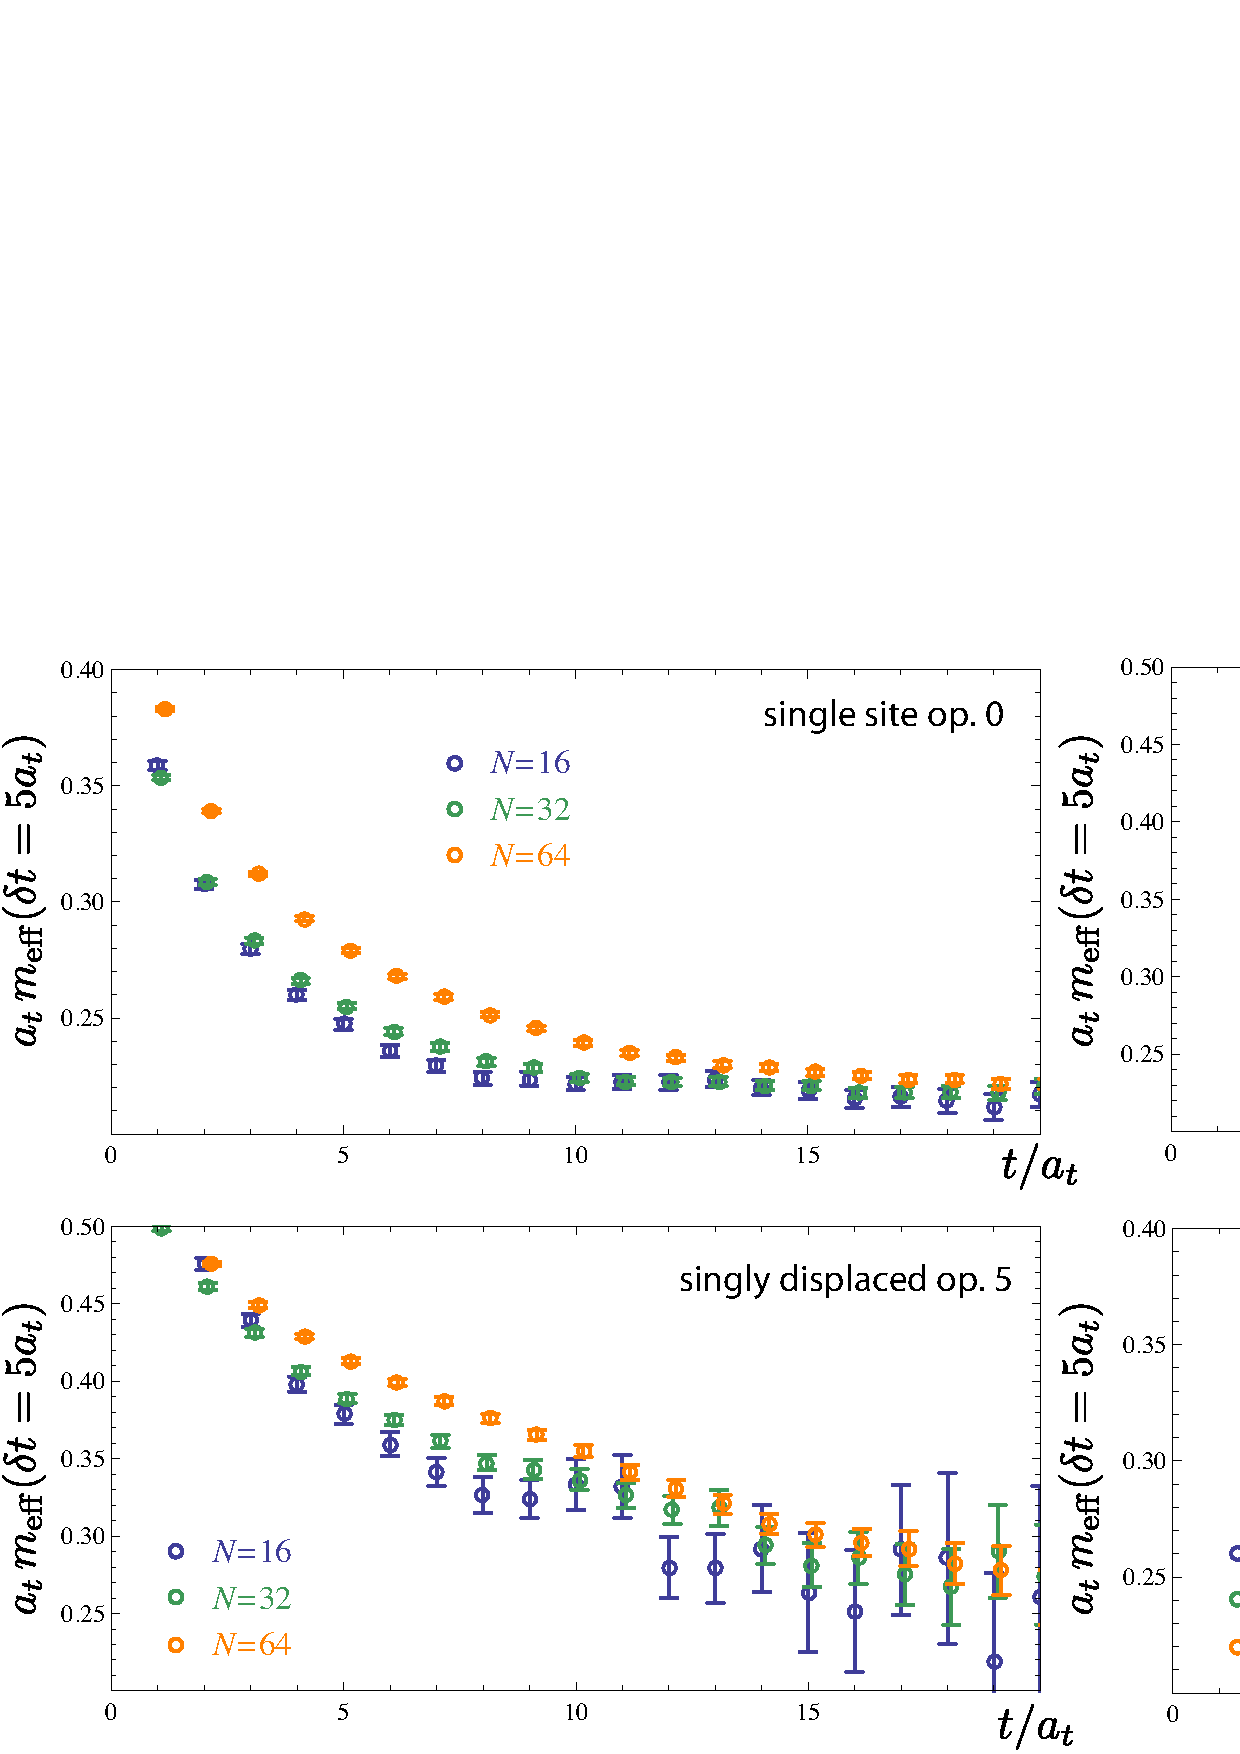
\includegraphics[width=0.9\textwidth]{images/baryon_meff.pdf}
\caption{\label{fig:baryon_meff_Nev}核子 $G_{1g}$ 道两个单格点与两个单位移
算符关联器的有效质量图。
}
\end{figure}
用式~\ref{noise} 对关联器噪信比建模
给出最佳拟合指数 $p \sim 1.1(2)$，再次表明：
增加矢量数降低噪声远快于简单统计标度。
用变分法 \cite{Michael:1985ne,Luscher:1990ck} 提取
了 $G_{1g}$ 谱中最低两个态的质量。
Figure~\ref{fig:baryon_Pmeff_Nev} 展示这些态的有效质量
对形成蒸馏算符所用本征矢量数的依赖关系。
发现质量彼此一致，且随矢量数增加统计精度提高。
\begin{figure}
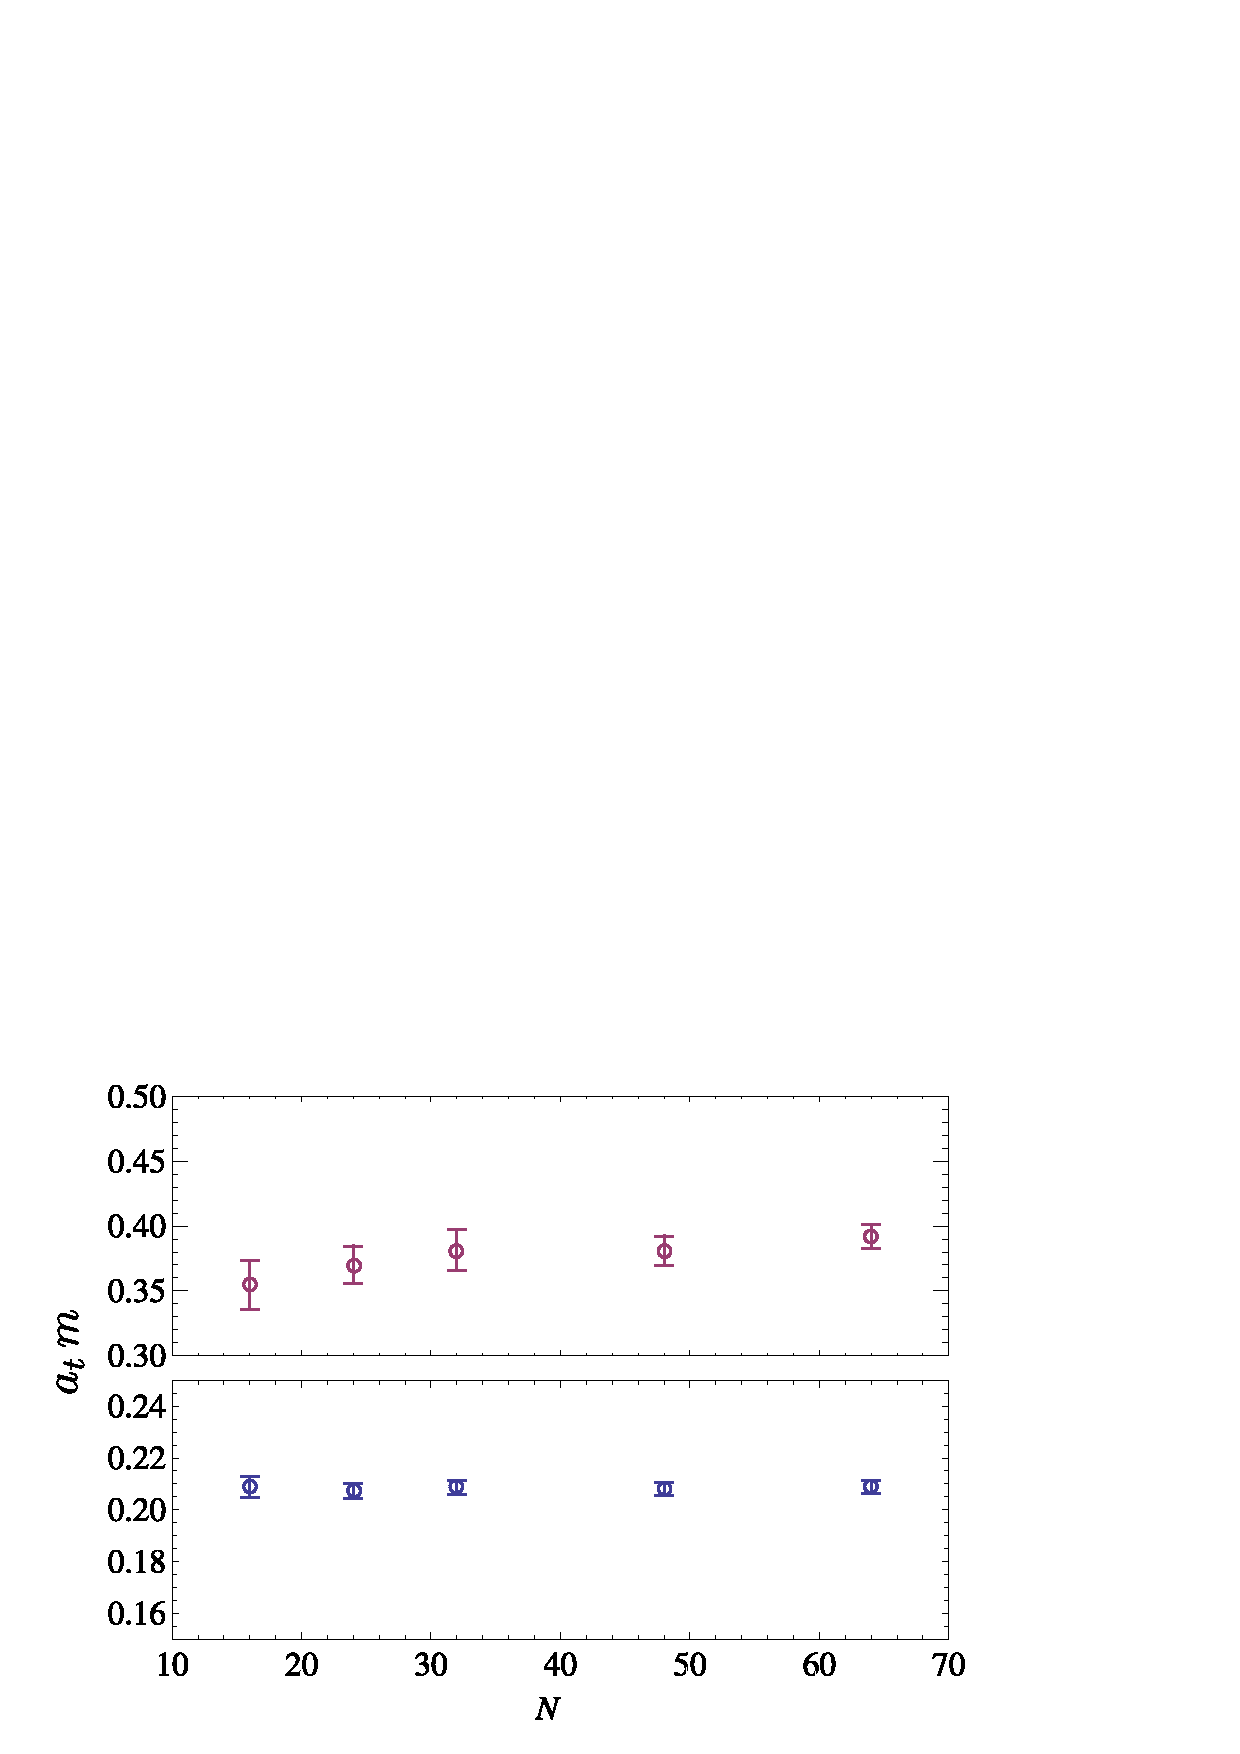
\includegraphics[width=0.5\textwidth]{images/G1g1NevPfitsT07_Ecomp2.pdf}
\caption{\label{fig:baryon_Pmeff_Nev} 第一激发态（上）与基态（下）的拟合能量
随 $N$ 的变化。
}
\end{figure}
Figure~\ref{fig:baryon_volume_meff_Nev} 展示了在 $16^3$ 与 $20^3$
格点上计算的对角有效质量。
加倍矢量数前后信号的相似性在这里不如介子情形明显。
\begin{figure}
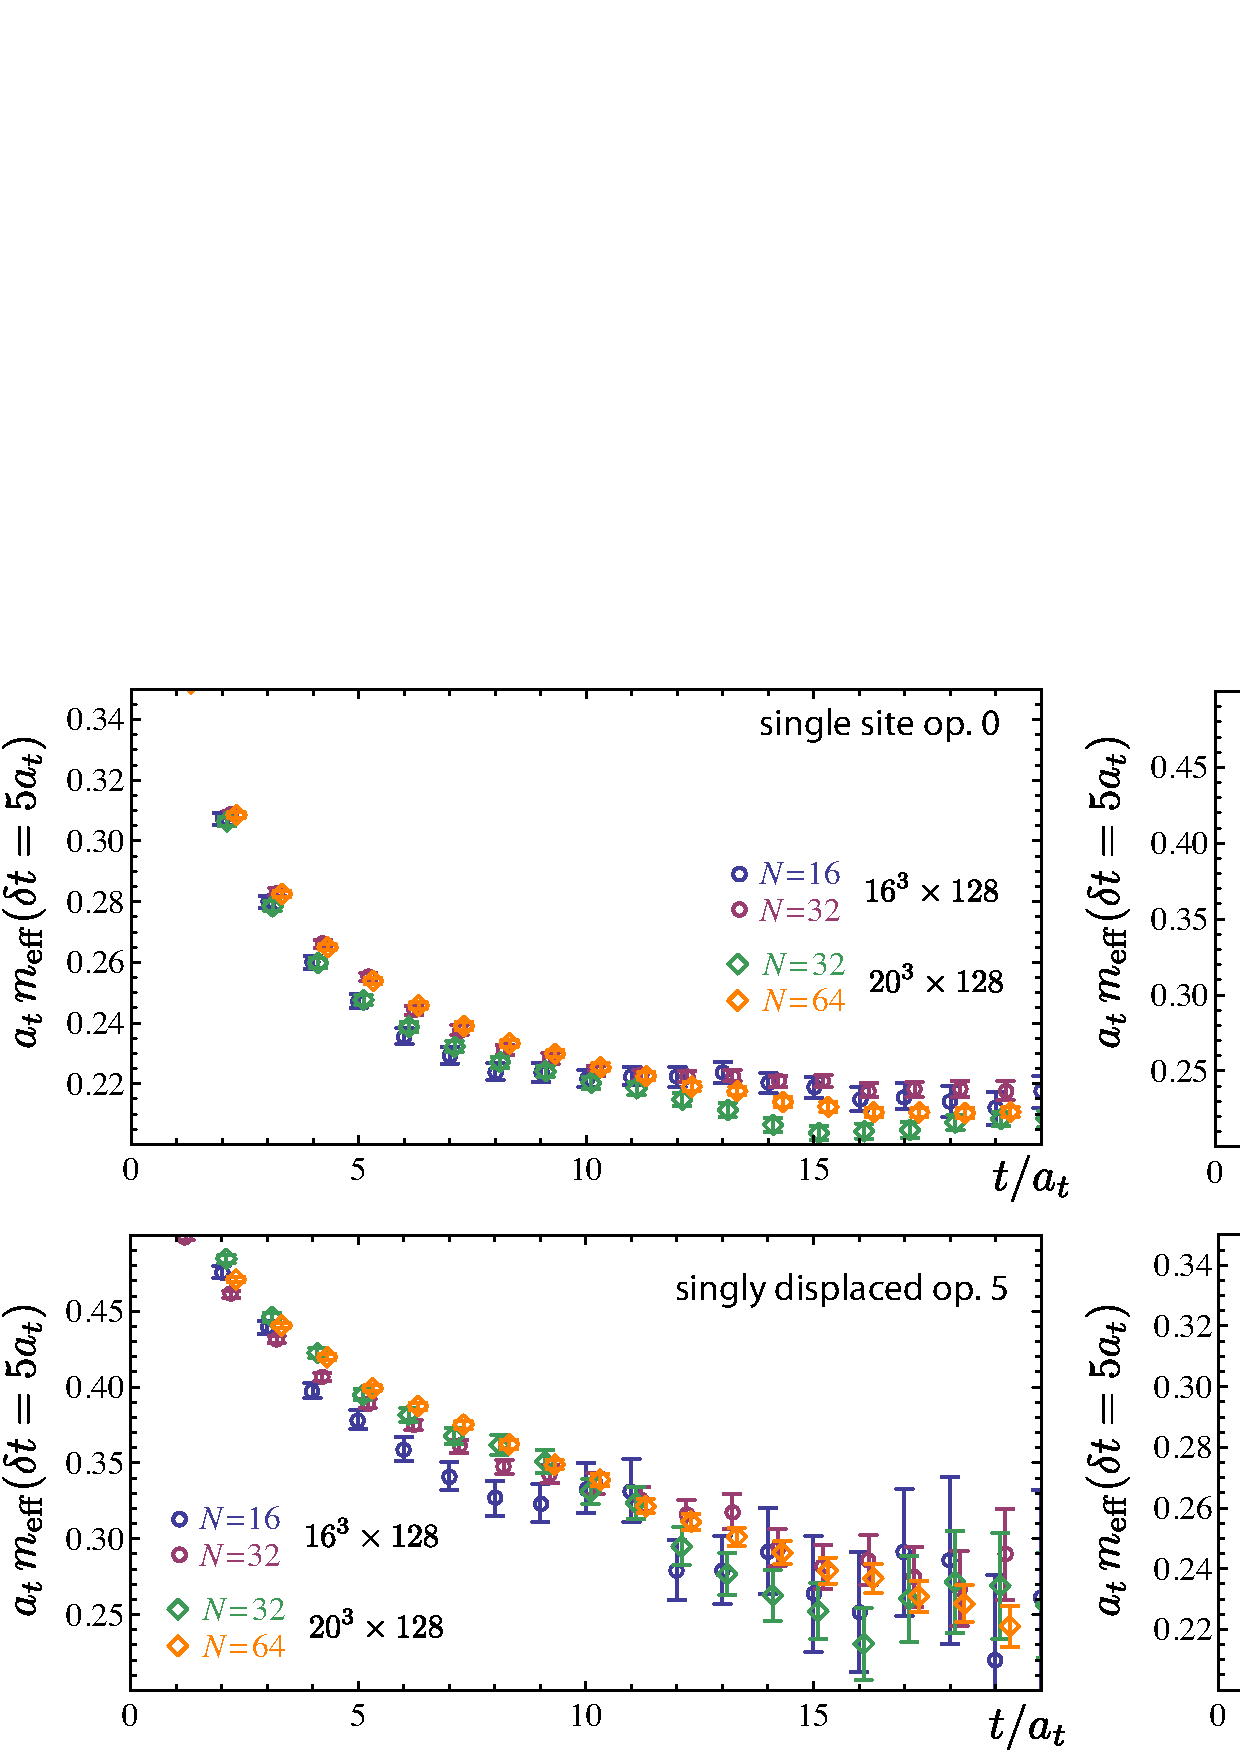
\includegraphics[width=0.9\textwidth]{images/baryon_meff_vol.pdf}
\caption{\label{fig:baryon_volume_meff_Nev}来自两个体积
$16^3\times128$ 与 $20^3\times128$ 的两个单格点与两个单位移算符
关联器的有效质量图
}
\end{figure}

\subsection{多介子关联函数}\label{subsec:results-multi-mesons}

定义蒸馏方法的主要动机之一是高效计算那些类似于多强子态——
组分强子具有确定动量——的产生算符的关联函数。
把这些态可靠而高效地纳入算符基，对处理散射与共振性质十分重要。
测试了最简单的情形：由式~\ref{eqn:multi_meson_quark_op} 构成的
同位旋二双 $\pi$ 介子态，其中单粒子算符
$M(\vec{p}_\mathrm{rel})$ 用局域算符 $\bar{u}\gamma_5 d$ 构造。
对此例考虑双 $\pi$ 算符
\begin{equation}
  \chi_{MM}(|\vec{p}_\mathrm{rel}|^2, t) =
    \sum_{k\in {\cal R}(\vec{p}_\mathrm{rel})}
   \chi_M(k,t) \, \chi_M(-k,t)
\end{equation}
总动量为零，单粒子算符具有相对动量 $\vec{p}_\mathrm{rel}$。
求和遍历经格点转动与 $\vec{p}_\mathrm{rel}$ 相联系的动量矢量集合
${\cal R}(\vec{p}_\mathrm{rel})$，以创造一个在转动下平凡变换的态；
于是该算符构成立方群的 $A_1$ 不可约表示。
在本检验中考虑了 $|\vec{p}_\mathrm{rel}|$ 从 0 到 $2 \times
\frac{2\pi}{L}$ 的所有取值，
对应 $\vec{p}_\mathrm{rel} =
\frac{2\pi}{L}\vec{n}$，其中 $\vec{n} \in \{(0,0,0), (1,0,0), (1,1,0), (1,1,1),
  (2,0,0)\}$。

在所有这些双 $\pi$ 算符之间形成一个 $5\times 5$ 关联矩阵，
并通过求解广义本征值问题将其对角化。
在 100 个组态上测得的最低三条主关联函数的有效质量
示于 Figure~\ref{fig:twopi}。即便统计量相对较低，
也清楚看到了第二激发态的信号信号。注意使用传统的 point-to-all
方法时，源算符不能投影到确定动量，
因此上述关联矩阵实际上无法构造。
\begin{figure*}
 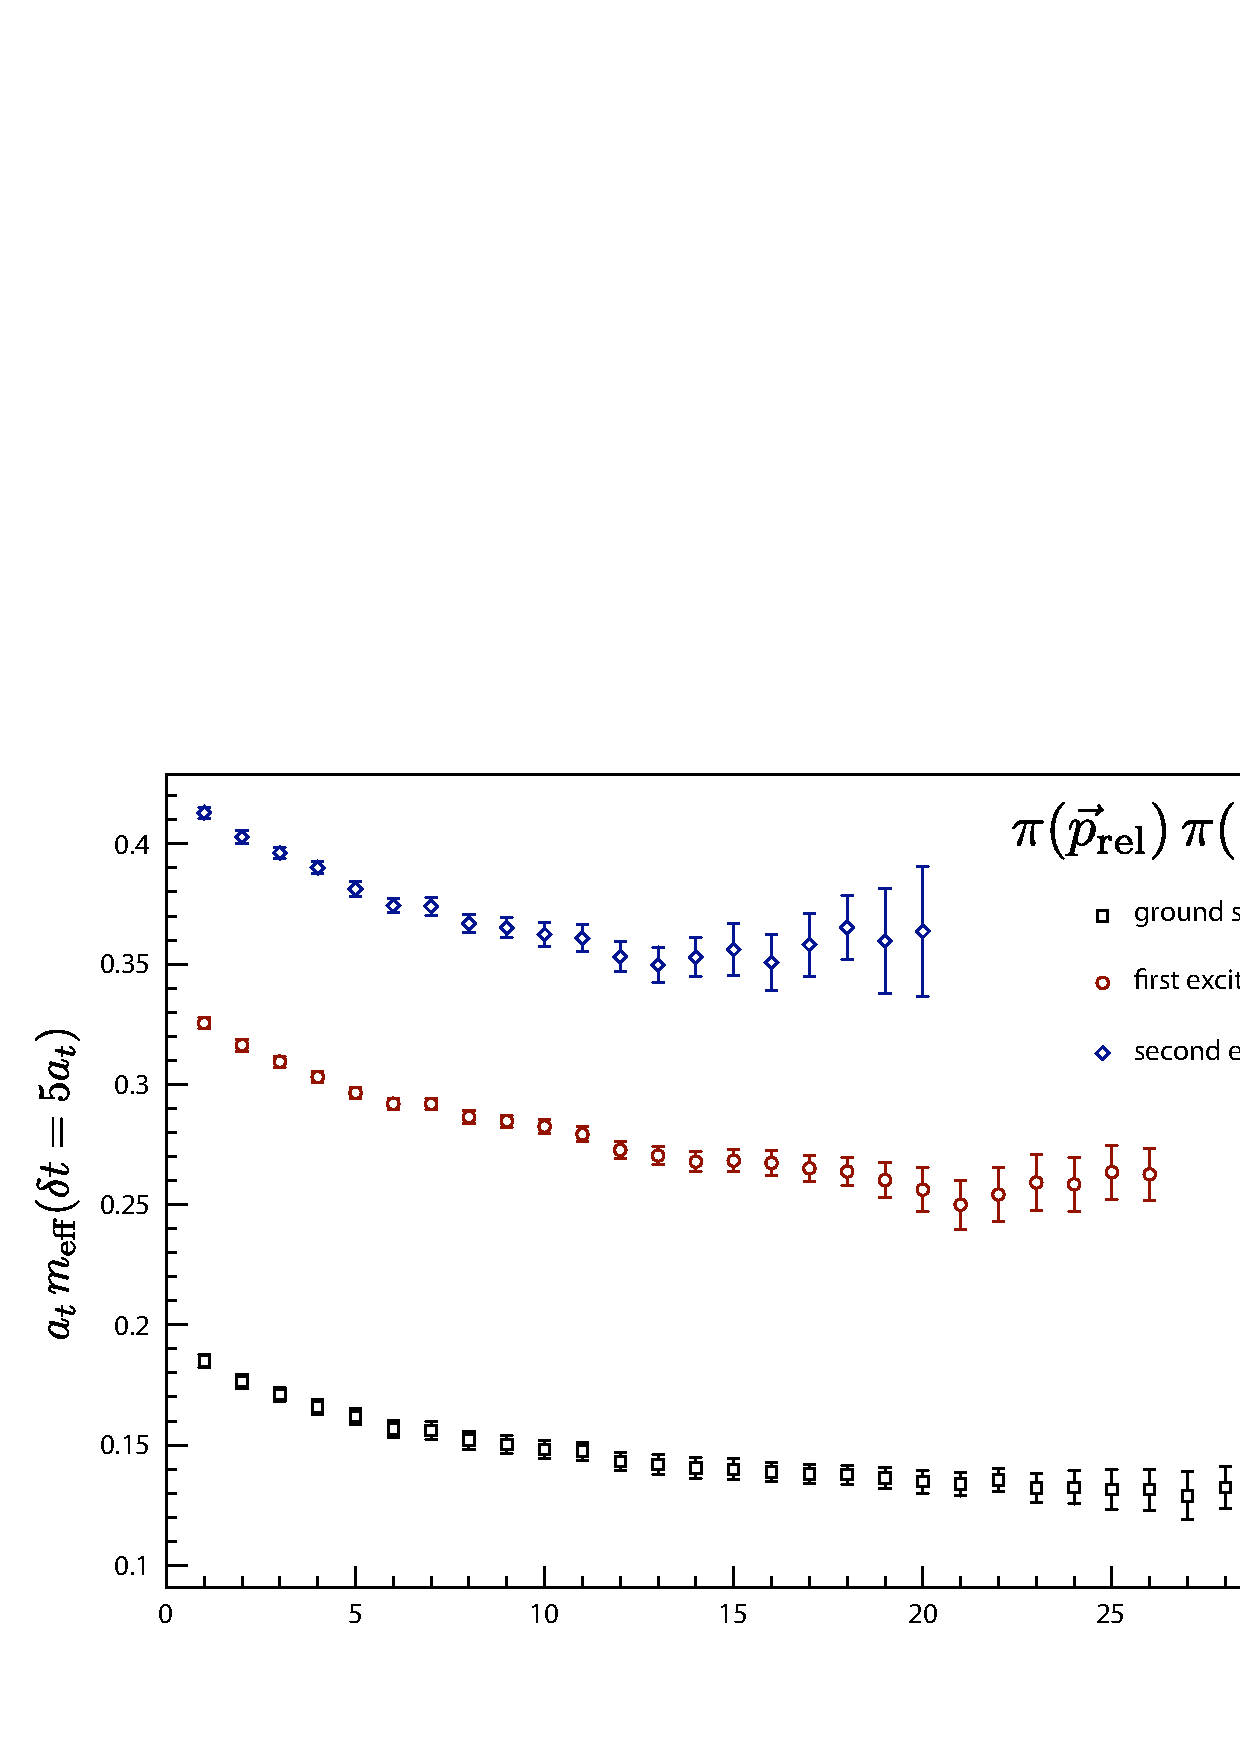
\includegraphics[width=10cm]{images/twopi.pdf}
\caption{\label{fig:twopi} $16^3\times 128$ 格点上同位旋二
$\pi(\vec{p}_\mathrm{rel})\pi(-\vec{p}_\mathrm{rel})$ 道（$A_1^{++}$）
前三条主关联器的有效质量（五时间片平移）。$5\times 5$ 关联矩阵
由 $|\vec{p}_\mathrm{rel}|^2 \in [0,4]$ 构成。关联器通过 $N=64$ 个矢量的
蒸馏在 100 个组态上构造。}
\end{figure*}
